\chapter{Literature Review}

% Once upon a time engineers and researchers believed... In this area of research, they used the following methods... \cite{jct2010}

% Write this section first as it will take you the longest. I suggest you start writing this as soon as you
% have done your initial research at the beginning of your project. You can then return to it once you
% have completed your work to edit and adjust it.

% A literature review forms the theoretical basis of your project. You need to read a large number of
% journal papers, sections in books, technical reports etc. relevant to your work at the start of project.
% This will give you a good idea of the field of research.

% When writing your review start of with the general concepts and move to the more specific aspects
% explaining the necessary theory as you go. This section is NOT a copy and paste from others work or a
% rewrite-but-change-one-word section. I suggest you read all your material, and then put it down and
% write this section, referring back to the work only when you need to check something.

% See your PCS textbook for more details on how to write a literature review.

% If you include a figure or a table in your text please see the example in Fig. \ref{fig:model} as to how to caption it.
% Please make sure that all text in your figures is readable and that you reference your figures if they are
% from another source.

% \begin{figure}[ht]
% \centering
% 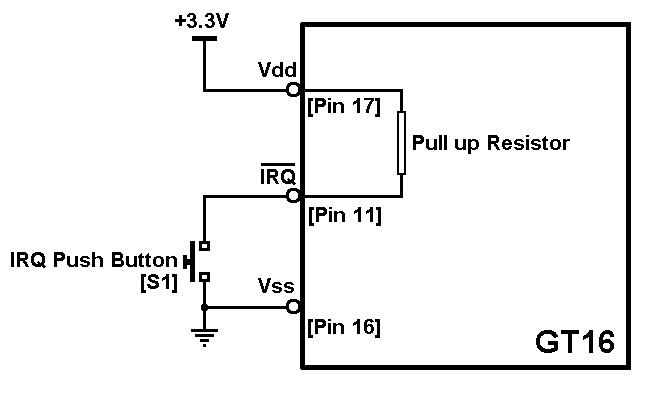
\includegraphics[width=0.7\textwidth]{graphics/model.png}
% \caption{A block diagram illustrating the connections to the IRQ pin on the MCS08GT16A microcontroller (Please
% note that your headings should be short descriptions of what is in the diagram not simply the figure title)}
% \label{fig:model}
% \end{figure}

\section{Tinkerkit Braccio arm for Arduno}
The Braccio arm has been used in similar projects to demonstrate teleoperation via intuitive control (natural human motions). An example uses an armband to measure the muscle contractions of a human arm \cite{bib:braccio_armband_demo}.

The Braccio arm has also been used in other projects. For a feeding-assistant, the engineers used Denavit-Hartenberg parameters and forward-kinematics to determine the position of the end-effector \cite{bib:braccio_feeding_assistant}. The Denavit-Hartenberg parameters used in the study are shown in \autoref{tab:lit_dh_parameters}.

\begin{table}[h!]
\centering
\caption{Denavit-Hartenberg parameters for Braccio arm}
\label{tab:lit_dh_parameters}
\begin{tabular}{|c|c|c|c|c|}
    \hline
    \textbf{i} & \textbf{$\alpha_{i-1}$ (degrees)} & \textbf{$r_{i-1}$ (inches)} & \textbf{$d_{i}$ (inches)} & $\theta_{i}$ (degrees) \\
    \hline \hline
    1 & 0 & 0 & 0 & $\theta_1$ \\
    \hline
    2 & 90 & 0 & 0 & $\theta_2$ \\
    \hline
    3 & 0 & 5 & 0 & $\theta_3$ \\
    \hline
    4 & 0 & 5 & 0 & $\theta_4$ \\
    \hline
    5 & 0 & 12 & 0 & $\theta_5$ \\
    \hline
\end{tabular}
\end{table}

There was a project involving the use of computer vision to control the Braccio arm \cite{bib:braccio_hand_gestures}. In this project, a camera connected to a Raspberry Pi would detect hand gestures (number of fingers being held up) from the user, and translate these into commands for the Braccio arm.

\section{Teleoperation}
Teleoperation has generally been in three categories \cite{bib:teleoperation_continuous_space}:
\begin{itemize}
    \item Joint mapping: Each joint of the slave device is mapped to a joint of the master device. This is only applicable if the kinematics are similar, which is not the case for a human arm and the Braccio arm.
    \item End-effector mapping: The end-effector of the slave device is mapped to the end-effector of the master, and the intermediate joints are determined with forward and inverse kinematics.
    \item Pose mapping: The general intention of the master device is mapped to the slave device.
\end{itemize}
The paper found that pose mapping, using a linear transformation in an intermediate space, was not only simpler to implement, but also more intuitive to use. The measure of "intuitiveness" comes from how quickly a novice was able to complete a task.

\section{Computer Vision}

The works of Moeslund and Granum \cite{bib:computer_vision_overview} summarises the advancements of computer vision in human tracking, from 1980 up till halfway through year 2000. The paper classifies human tracking into three applications; surveillance, control and analysis. From the descriptions given, control is what's relevant to this project.

The paper lists some common assumptions made in the context of computer vision. Computer vision isn't the focus of this project, so as many assumptions as applicable will be made, namely:
\begin{itemize}
    \item The subject (human arm) remains inside the workspace
    \item No camera motion
    \item Only one person in the workspace at the time
    \item No occlusion
    \item The motion pattern of the subject is known
    \item Minimal changes to lighting
    \item Static/uniform background
    \item Known camera parameters
\end{itemize}
That being the case, robustness of a tracking algorithm is not as much of a priority, compared to accuracy and speed.

The paper also discusses different ways of modelling the hand, from different abstraction methods. The stick-figure model, with joint-abstraction stands out, because it can most easily be translated into a corresponding pose for the Braccio arm.
